% Preamble

% use the beamer document class
\documentclass[hyperref={pdfpagelabels=false}, 14pt]{beamer}
% Text in square brackets is to avoid the warning: Package hyperref Warning: Option `pdfpagelabels’ is turned off (hyperref) because \thepage is undefined. Hyperref stopped early
% See: http://texblog.net/latex-archive/presentations/beamer-warnings/

% to set up the beamer class to use another colour shade, use these lines instead of the one above
%\documentclass[xcolor=dvipsnames]{beamer} 
%\usecolortheme[named=Brown]{structure}

% use Latin Modern fonts
% This also avoids the warnings: LaTeX Font Warning: Font shape `OT1/cmss/m/n’ in size <4> not available (Font) size <5> substituted on input line 6. and: LaTeX Font Warning: Size substitutions with differences  (Font) up to 1.0pt have occurred.
\usepackage{lmodern}

%\usepackage[T1]{fontenc}
%\usepackage[T1]{tipa}
%\usepackage[tipa]{ucs}
\usepackage[utf8x]{inputenc}  % required to allow accented characters like â to appear properly
\usepackage{textcomp}  % to allow arrows
\usepackage{fancyvrb}  % to allow tabs in verbatim text

% use Times New Roman as the default font
%\renewcommand{\rmdefault}{ptm}

% replace the theme lines below with the following line to get rid of most of the colours for handouts
%\usetheme{default}

%\usetheme{Warsaw}
% comment out this line to get a white background and black text on the slide body
%\usecolortheme{albatross}

%\beamertemplateshadingbackground{blue!70}{blue!100}  % gradient full-blue to partial-blue

%\setbeamercolor{structure}{fg=blue!30}
%\setbeamercolor{normal text}{fg=blue!30}
\setbeamertemplate{background canvas}{
\includegraphics [width=\paperwidth,height=\paperheight]{mainpage.jpg}}
%\setbeamertemplate{footline}{\insertframenumber/ \inserttotalframenumber}
\setbeamertemplate{navigation symbols}{}  % hide navigation buttons 

% specify the details to appear on the title page
\title[Constraint grammar in the Bangor Autoglosser]{\newline\newline\newline\newline \normalsize Using constraint grammar \\ in the Bangor Autoglosser\\to disambiguate multilingual spoken text}
\author{Kevin Donnelly and Margaret Deuchar}
\institute{ESRC Centre for Research on Bilingualism, Bangor, Wales}
\date{}

\begin{document}

% build title page
{ % brace to limit the scope of \setbeamertemplate 
\setbeamertemplate{navigation symbols}{}  % hide navigation buttons 
\setbeamertemplate{background canvas}{
\includegraphics [width=\paperwidth,height=\paperheight]{titlepage.jpg}}
\maketitle
} % closing brace

%============================


% Multilingual discourse is far more common than has been assumed in classical linguistics
% Bangor Autoglosser seems to be the first POS-tagger for Welsh


\section{Background}


\begin{frame}
\frametitle{}
\begin{center}
\begin{huge} Background \end{huge}
\end{center}
\end{frame}


\subsection{The Centre and the corpora}


\begin{frame}
\frametitle{\begin{small}\insertframenumber/\inserttotalframenumber\end{small} The Centre}
\begin{itemize}
\item ESRC Centre for Research in Bilingualism
\item Established January 2007
% First research centre in the UK to focus specifically on bilingualism
\item Five research themes
% Neuroscience, experimental research, ethnography, speech
\item Corpus-based research
\item \textbf{bilingualism.bangor.ac.uk}
\end{itemize}
\end{frame}


\begin{frame}
\frametitle{\begin{small}\insertframenumber/\inserttotalframenumber\end{small} Bangor corpora}
\begin{center}
\begin{tabular}{ccccc}
& \begin{small}\textit{Chats}\end{small} & \begin{small}\textit{Hours}\end{small} & \begin{small}\textit{Words}\end{small} & \begin{small}\textit{Date}\end{small} \\
\cline{1-5}\noalign{\smallskip}
\textbf{Welsh-English} & 69 & 40 & 456k & 2009 \\
(Siarad) & & & \\
\textbf{Welsh-Spanish} & 32 & 20 & 161k & 2011 \\
(Patagonia) & & & \\
\textbf{Spanish-English} & 31 & 20 & 126k & 2011 \\
(Miami) & & & \\
\hline\noalign{\smallskip}
& \textbf{132} & \textbf{80} & \textbf{743k} \\
\multicolumn{5}{l}{} \\
\multicolumn{5}{l}{All available under the GPL.}
\end{tabular}
\end{center}
\end{frame}


\begin{frame}
\frametitle{\begin{small}\insertframenumber/\inserttotalframenumber\end{small} The conversations}
\begin{itemize}
\item Transcribed using the CLAN format
% Fairly high-level system
\item \textbf{childes.psy.cmu.edu/clan}
% Originally developed to study language acquisition
\item Standard orthography
% Recordings available, so phonetic transcription could be done if required
% Main concern is use of two langauges by a bilingual speakers
  \begin{itemize}
  \item Elisions spelled out for Welsh:
  \item \textbf{mae'n fawr} (it's big) \textrightarrow \textbf{mae (y)n fawr}
  % Helpful for the dictionary
  \end{itemize}
\item Gloss added
\item Free translation in English added
\end{itemize}
\end{frame}


\subsection{Corpus layout}


\begin{frame}
\frametitle{\begin{small}\insertframenumber/\inserttotalframenumber\end{small} Sample utterances}
\begin{footnotesize}

\textbf{*SER:}   dw@1 i@1 (y)n@1 hopeless@2 efo@1 tynnu@1 llun@1 . \%snd:"deuchar1"\_72848\_73881

\textit{\%gls:}   be.1S.PRES PRON.1S PRT hopeless with take.NONFIN picture

\textit{\%eng:}   I'm hopeless at drawing

\textbf{*MYF:}   +$<$ \&=laugh . \%snd:"deuchar1"\_73196\_73881

\textbf{*SER:}   dw@1 i@1 (y)n@1 tynnu@1 llun@1 i@1 [/] i@1 (y)r@1 plant@1 $<$i@1 plant@1$>$ [//] $<$i@1 (y)r@1$>$ [//] \# i@1 er@0 \&h Helen@0 a@1 Susanna@0 a@1 +/. \%snd:"deuchar1"\_73881\_79477

\textit{\%gls:}   be.1S.PRES PRON.1S PRT take.NONFIN picture for for DET children for children for DET for IM Helen and Susanna and

\textit{\%eng:}   I draw a picture for \dots for the children, for, er, Helen and Susanna and \dots

\end{footnotesize}
\begin{small}
\hfill\textit{(Siarad corpus, deuchar1)}
\end{small}
% Hesitation markers, delivery hints, elision
\end{frame}


\begin{frame}
\frametitle{\begin{small}\insertframenumber/\inserttotalframenumber\end{small} Utterance format}
\begin{center}
\begin{small}

\begin{tabular}{p{3cm}p{6cm}}
\multicolumn{2}{p{9cm}}{\textit{*SER dw@1 i@1 (y)n@1 hopeless@2 efo@1 tynnu@1 llun@1 . \%snd:"deuchar1"\_72848\_73881}} \\
\hline\noalign{\smallskip}
\textbf{Speaker} & *SER \\
\hline\noalign{\smallskip}
\textbf{Utterance} & dw@1 i@1 (y)n@1 hopeless@2 efo@1 tynnu@1 llun@1 . \\
\hline\noalign{\smallskip}
\textbf{Language tags} & 1=Welsh, 2=English, 0=undetermined \\
% Uses old coding 
\hline\noalign{\smallskip}
\textbf{Audio location} & \%snd:"deuchar1"\_72848\_73881 \\
\hline\noalign{\smallskip}
\textbf{Manual gloss} & be.1S.PRES PRON.1S PRT hopeless with take.NONFIN picture
% Provides lexemes and POS tags, but mainly for verbs
\end{tabular}
\end{small}
\end{center}
\end{frame}


\begin{frame}
\frametitle{\begin{small}\insertframenumber/\inserttotalframenumber\end{small} Why?}
\begin{itemize}
\item Examine how language is actually used
\item Differences between spoken language and formal written language
\item Sociolinguistic variation -- what is used where by whom
\item Balance between languages in bilingual usage
\item How one language handles lexical items from the other
    \begin{itemize}
    \item Welsh loan-verbs such as \textit{textio} (to text) behave more like ordinary Welsh verbs the more frequent they are
    \end{itemize}

\end{itemize}
\end{frame}


\subsection{Glossing}


\begin{frame}
\frametitle{}
\begin{center}
\begin{huge} Glossing \end{huge}
\end{center}
\end{frame}


\begin{frame}
\frametitle{\begin{small}\insertframenumber/\inserttotalframenumber\end{small} Why gloss?}
\begin{itemize}
\item Lexemes and part-of-speech (POS) tags:
    \begin{itemize}
    \item Help non-native speakers parse the conversation
    \item Allow further analysis - morphological, syntactic, sociolinguistic
    % Useful to provide if it can be provided
\end{itemize}
\item Difficulties:
    \begin{itemize}
    \item Time-consuming and tedious
    \item Inconsistency and errors \\ (\textit{ychydig} -- ``a\_bit''/``a\_little'')
    % Difficult to do automated selection later
    \item Tag choice difficult to revise later
    \end{itemize}
\end{itemize}
\end{frame}


\begin{frame}
\frametitle{\begin{small}\insertframenumber/\inserttotalframenumber\end{small} Automation}
\begin{itemize}
\item April 2010
\item Explore automation to address difficulties above
\item Move towards more granular POS information
\item Welsh \textrightarrow Spanish \textrightarrow English
\item Accuracy reflects timespend: \\
99\% for Welsh, and 95\% for English.
%Spanish in between
\item Work in progress
\end{itemize}
\end{frame}


\section{Method}


\subsection{Background}


\begin{frame}
\frametitle{\begin{small}\insertframenumber/\inserttotalframenumber\end{small} Why another wheel?}
\begin{itemize}
\item CLAN tagging system
% MOR only available for 11 languages - Cantonese (52m), Danish (5m), Dutch (22m), English (328m), French (68m), German (90m), Hebrew (5m), Japanese(122m), Italian (62m), Mandarin (840m), Spanish (329m)
% POST only available for 4 of these: English, Chinese, Japanese, Spanish
    \begin{itemize}
    \item For 11 languages $>$ 5m speakers
    \item Requires one pass for each language
    \item Can't mix language context
    \item Vocabulary stored in a number of files
    \item Disambiguation for only 4 languages
    \end{itemize}
\item Toolbox
% Apps like Toolbox are more for ongoing work discovering the structure of a language
% Not really appropriate here - needs to be scriptable, otherwise too slow
\item No automated system for small languages
\end{itemize}
\end{frame}   

\begin{frame}
\frametitle{\begin{small}\insertframenumber/\inserttotalframenumber\end{small} Pilot project}
\begin{itemize}
\item Test project over two weeks:
    \begin{itemize}
    \item No disambiguation
    \item Write out entries from Spanish dictionary
    \item \textbf{apertium.org}
    \item Compare them with MOR output
    \item Write out entries from Welsh dictionary
    \item \textbf{eurfa.org.uk}
    \end{itemize}
% Apps like Toolbox are more for ongoing work discovering the structure of a language
% Not really appropriate here - needs to be scriptable, otherwise too slow
\item Good results
\item Needed a way to disambiguate - enter CG!
% Before I do that, though, I'll just give a few more details about the dictionary lookup
\end{itemize}
\end{frame} 


\subsection{Dictionaries}


\begin{frame}
\frametitle{}
\begin{center}
\begin{huge} Dictionaries \end{huge}
\end{center}
\end{frame}



\begin{frame}
\frametitle{\begin{small}\insertframenumber/\inserttotalframenumber\end{small} Dictionaries}
\begin{itemize}
\item Derived from GPL or PD resources
% Eurfa, Apertium, Kevin Atkinson/Grady Ward
\item One database table
\item Words, not morphemes
\item Easily presented in a spreadsheet
% May be less forbidding than a database to most linguists
\item Easy to update
\item Easy to get started
% Any basic wordlist will do
\end{itemize}
\end{frame}


\begin{frame}
\frametitle{\begin{small}\insertframenumber/\inserttotalframenumber\end{small} Welsh dictionary}
\begin{center}
\begin{small}
\begin{tabular}{ccccccc}
\textit{surface} & \textit{lemma} & \textit{enlemma} & \textit{pos} & \textit{gender} & \textit{number} & \textit{tense} \\
\hline\noalign{\smallskip}
\textbf{bara} & bara & bread & n & m & sg & \\
\hline\noalign{\smallskip}
\textbf{cathod} & cath & cat & n & f & pl & \\
\hline\noalign{\smallskip}
\textbf{mynd} & mynd & go & v & & & infin \\
\hline\noalign{\smallskip}
\textbf{aeth} & mynd & go & v & & 3s & past \\
\hline\noalign{\smallskip}
\textbf{hapus} & hapus & happy & adj & &  & \\
\hline\noalign{\smallskip}
\textbf{rhywsut} & rhywsut & somehow & adv & & & \\
\hline\noalign{\smallskip}
\textbf{heb} & heb & without & prep & & & \\
\hline\noalign{\smallskip}
\end{tabular}
% Quite simple
% Easily accessible to non-CS people
\end{small}
\end{center}
\end{frame}


\begin{frame}
\frametitle{\begin{small}\insertframenumber/\inserttotalframenumber\end{small} Spanish dictionary}
\begin{center}
\begin{small}
\begin{tabular}{ccccccc}
\textit{surface} & \textit{lemma} & \textit{enlemma} & \textit{pos} & \textit{gender} & \textit{number} & \textit{tense} \\
\hline\noalign{\smallskip}
\textbf{perro} & perro & dog & n & m & sg & \\
\hline\noalign{\smallskip}
\textbf{canciones} & canción & song & n & f & pl & \\
\hline\noalign{\smallskip}
\textbf{empezar} & empezar & start & v & & & infin \\
\hline\noalign{\smallskip}
\textbf{empieza} & empezar & start & v & & 23s & pres \\
\hline\noalign{\smallskip}
\textbf{empieza} & empezar & start & v & & 2s & imper \\
\hline\noalign{\smallskip}
\textbf{rojo} & rojo & red & adj & m & sg & \\
\hline\noalign{\smallskip}
\textbf{rojas} & rojo & red & adj & f & pl & \\
\hline\noalign{\smallskip}
\textbf{por} & por & for & prep & & & \\
\hline\noalign{\smallskip}
\end{tabular}
% Quite simple
% Easily accessible to non-CS people
\end{small}
\end{center}
\end{frame}


\begin{frame}
\frametitle{\begin{small}\insertframenumber/\inserttotalframenumber\end{small} English dictionary}
\begin{center}
\begin{small}
\begin{tabular}{ccccccc}
\textit{surface} & \textit{lemma} & \textit{pos} & \textit{number} & \textit{tense} \\
\hline\noalign{\smallskip}
\textbf{break} & break & sv & & infin \\
\hline\noalign{\smallskip}
\textbf{broke} & break & av & & past \\
\hline\noalign{\smallskip}
\textbf{broken} & break & av & & pastpart \\
\hline\noalign{\smallskip}
\textbf{car} & car & n & sg & \\
\hline\noalign{\smallskip}
\textbf{quick} & adj & & & \\
\hline\noalign{\smallskip}
\textbf{by} & by & prep & & \\
\hline\noalign{\smallskip}
\textbf{which} & which & rel & & \\
\hline\noalign{\smallskip}
\end{tabular}
% Simpler layout - one entry for ``break'' a clean break, break the bank, they break the rules
% Gender field is available, but not really used.  Enlemma just repeats surface.
\\ \medskip
\begin{footnotesize}\textit{breaks, breaking, cars, quickly} are derived during lookup\end{footnotesize}
\end{small}
\end{center}
\end{frame}


\begin{frame}
\frametitle{\begin{small}\insertframenumber/\inserttotalframenumber\end{small} Language differences}
\begin{itemize}
\item Spanish and Welsh
    \begin{itemize}
    \item Inflected (Welsh less so than it was)
    \item Surface forms give clues about the POS
    \end{itemize}
\item English 
    \begin{itemize}
    \item Analytic
    \item Homophonous surface forms
    \item POS defined by role in the sentence
    \item \textbf{break}
        \begin{itemize}
        \item \textit{a clean break} (noun)
        \item \textit{break the mould!} (imperative)
        \item \textit{to break a habit} (infinitive)
        \item \textit{they break everything} (present)
        \end{itemize}
    \end{itemize}
\end{itemize}
\end{frame}


\subsection{Import}


\begin{frame}
\frametitle{}
\begin{center}
\begin{huge} Import \end{huge}
\end{center}
\end{frame}


\begin{frame}
\frametitle{\begin{small}\insertframenumber/\inserttotalframenumber\end{small} Import the chat file}
\begin{itemize}
% Don't need to spend too much time on this
\item PHP script reads each line into a PostgreSQL database table
\item Selects the utterance and discards markers
\item Splits the cleaned utterance into words
\item Puts them into another database table
%\item Handles 4 different language-tagging systems
% Different transcribers have worked on the corpora over the 5-year period
% CLAN itself has changed its system
% Earlier sample showed 0,1,2 for language-tags
% Current one only tags non-default items with the ISO 3-letter tag
\end{itemize}
\end{frame}


\begin{frame}
\frametitle{\begin{small}\insertframenumber/\inserttotalframenumber\end{small} Utterance-table fields}
\begin{small}
\begin{itemize}\setlength{\itemsep}{-1mm}
\item utterance\_id
\item filename
\item speaker
\item surface
\item startpoint
\item endpoint
\item duration
\item manual glosses (if present)
\item English translation (if present)
\item comments (if present)
\item precode (if present -- marks entire utterances in the least-frequent language)
% 
\end{itemize}
\end{small}
\end{frame}


\begin{frame}
\frametitle{\begin{small}\insertframenumber/\inserttotalframenumber\end{small} Word-table fields}
\begin{small}
\begin{itemize}\setlength{\itemsep}{-1mm}
\item word\_id
\item utterance\_id
\item location of the word in the utterance
\item surface
\item automatic glosses
\item manual glosses (if present)
\item language id
\item speaker
\item filename
% Once the words are in this table, they are ready for lookup against the dictionary
% Followed by disambiguation by CG
\end{itemize}
\end{small}
\end{frame}


\begin{frame}
\frametitle{\begin{small}\insertframenumber/\inserttotalframenumber\end{small} The words table}
  \begin{figure}[h]
  \centering
  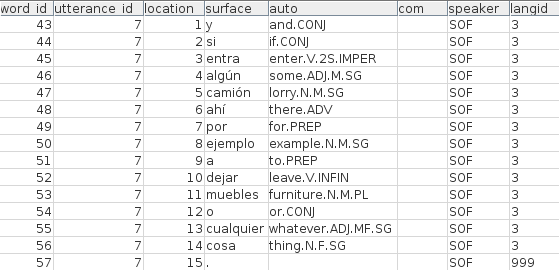
\includegraphics[width=\textwidth]{words_table.png}
  \end{figure}
  % Spanish sentence from the Miami corpus.
  % At this stage the autogloss field would be empty - that is what we're going to add now.
\end{frame}


\begin{frame}
\frametitle{\begin{small}\insertframenumber/\inserttotalframenumber\end{small} Lookup}
\begin{itemize}
\item Each word is looked up against the appropriate dictionary
\item Uses the language id assigned to the word
\item Writes out all ``hits'' in the CG input format
% 
\end{itemize}
\end{frame}


\begin{frame}
\frametitle{\begin{small}\insertframenumber/\inserttotalframenumber\end{small} Segmentation}
\begin{itemize}
\item Lookup also does some basic segmentation
\item Minimises number of dictionary entries \\ (\textbf{break} above)
\item Welsh: mutated words are tagged
% I better summarise what mutation is
    \begin{itemize}
    \item thad \textrightarrow tad (\textit{father}) + am
    \item gael \textrightarrow cael (\textit{get}) + am
    \end{itemize}
\item Spanish: clitic pronouns are tagged  
    \begin{itemize}
    \item ponerle \textrightarrow poner (\textit{put}) + le[pron.mf.3s]
    \item déjanos \textrightarrow dejar (\textit{leave})+ nos[pron.mf.1p]
    \end{itemize}
\end{itemize}
\end{frame}


\begin{frame}
\frametitle{\begin{small}\insertframenumber/\inserttotalframenumber\end{small} English Segmentation}
\begin{itemize}
\item Elisions are tagged
    \begin{itemize}
    \item gonna \textrightarrow go \# to.prep
    \item we're \textrightarrow we \# be.v.pres
    \end{itemize}
\item Plurals or verbs (3p sg pres) are tagged
    \begin{itemize}
    \item breaks \textrightarrow break \# pv
    \end{itemize}
\item Adjectives or verbs (past or pastpart) are tagged
    \begin{itemize}
    \item constructed \textrightarrow construct \# av
    \end{itemize}
\item Adjectives, nouns or verbs (prespart) are tagged
    \begin{itemize}
    \item thinking \textrightarrow think \# asv
    \end{itemize}
\end{itemize}
\end{frame}


\begin{frame}
\frametitle{\begin{small}\insertframenumber/\inserttotalframenumber\end{small} Mutation}
\begin{itemize}
\item \textbf{tad} (father)
    \begin{itemize}
    \item \textbf{ei \underline{d}ad} (\underline{his} father)
    \item \textbf{ei \underline{th}ad} (\underline{her} father) 
    \end{itemize}
\item \textbf{marw} (die, dead)
    \begin{itemize}
    \item \textbf{mae o'n \underline{m}arw} (he is dying)
    \item \textbf{mae o'n \underline{f}arw} (he is dead)
    \end{itemize}
\item direct object following a verb
    \begin{itemize}
    \item \textbf{Mi werthodd y ffermwr y \underline{m}ochyn}\\ (The farmer sold the pig)
    \item \textbf{Mi werthodd y ffermwr \underline{f}ochyn}\\ (The farmer sold a pig)
    \end{itemize}
\end{itemize}
\end{frame}


\begin{frame}[fragile]
\frametitle{\begin{small}\insertframenumber/\inserttotalframenumber\end{small} Welsh before CG}
\begin{scriptsize}
\begin{BVerbatim}
"<ddim>"
    "dim"  {96,1} [cy] n m sg :nothing: [208789] + sm
    "dim"  {96,1} [cy] adv :not: [204176] + sm
"<yn>"
    "yn"  {96,2} [cy] stat :stative: [200654]
    "yn"  {96,2} [cy] prep :in: [204430]
    "gan"  {96,2} [cy] prep :with: [196964] + sm
"<gynnar>"
    "cynnar"  {96,3} [cy] adj :early: [209212] + sm
"<iawn>"
    "iawn"  {96,4} [cy] adv :OK: [207540]
    "iawn"  {96,4} [cy] adv :very: [203775]
"<.>"
\end{BVerbatim}
\\ \hfill\textit{(Miami corpus, sastre1)}
\end{scriptsize}
\end{frame}


\begin{frame}[fragile]
\frametitle{\begin{small}\insertframenumber/\inserttotalframenumber\end{small} Welsh after CG}
\begin{scriptsize}
\begin{BVerbatim}
"<ddim>"
    "dim" {96,1} [cy] adv :not: [204176] + sm
"<yn>"
    "yn" {96,2} [cy] stat :stative: [200654]
"<gynnar>"
    "cynnar" {96,3} [cy] adj :early: [209212] + sm
"<iawn>"
    "iawn" {96,4} [cy] adv :very: [203775]
"<.>"
\end{BVerbatim}
\\ \hfill\textit{(Patagonia corpus, patagonia1)}
\end{scriptsize}
\end{frame}
 

\begin{frame}[fragile]
\frametitle{\begin{small}\insertframenumber/\inserttotalframenumber\end{small} Spanish before CG}
\begin{scriptsize}
\begin{BVerbatim}
"<y>"
    "y"  {122,1} [es] conj :and: [118037]
"<ahora>"
    "ahora"  {122,2} [es] adv :now: [6292]
"<vamos>"
    "ir"  {122,3} [es] v 1p pres :go: [115789]
"<a>"
    "a"  {122,4} [es] prep :to: [1]
"<hacerle>"
    "hacer"  {122,5} [es] v infin :do: [62577] + le[pron.mf.3s]
"<el>"
    "el"  {122,6} [es] det.def m sg :the: [45129]
"<baño>"
    "baño"  {122,7} [es] n m sg :bathroom: [16011]
    "bañar"  {122,7} [es] v 1s pres :bathe: [16010]
"<.>"
\end{BVerbatim}
\\ \hfill\textit{(Patagonia corpus, patagonia1)}
\end{scriptsize}
\end{frame}


\begin{frame}[fragile]
\frametitle{\begin{small}\insertframenumber/\inserttotalframenumber\end{small} Spanish after CG}
\begin{scriptsize}
\begin{BVerbatim}
``<y>"
    "y" {122,1} [es] conj :and: [118037]
"<ahora>"
    "ahora" {122,2} [es] adv :now: [6292]
"<vamos>"
    "ir" {122,3} [es] v 1p pres :go: [115789]
"<a>"
    "a" {122,4} [es] prep :to: [1]
"<hacerle>"
    "hacer" {122,5} [es] v infin :do: [62577] + le[pron.mf.3s]
"<el>"
    "el" {122,6} [es] det.def m sg :the: [45129]
"<baño>"
    "baño" {122,7} [es] n m sg :bathroom: [16011]
"<.>"
\end{BVerbatim}
\\ \hfill\textit{(Miami corpus, sastre1)}
\end{scriptsize}
\end{frame}


\begin{frame}[fragile]
\frametitle{\begin{small}\insertframenumber/\inserttotalframenumber\end{small} English before CG}
\begin{scriptsize}
\begin{verbatim}
"<it's>"
    "it"  {545,1} [en] pron.sub 3s :it: [130342] # gb
"<coming>"
    "come"  {545,2} [en] sv infin :come: [82193] # asv
"<out>"
    "out"  {545,3} [en] adv :out: [157287]
"<on>"
    "on"  {545,4} [en] prep :on: [156077]
"<D_V_D>"
    "D_V_D"  {545,5} [en] name
"<then>"
    "then"  {545,6} [en] adv :then: [208154]
"<.>"
\end{verbatim}
\hfill\textit{(Miami corpus, herring7)}
\end{scriptsize}
\end{frame}


\begin{frame}[fragile]
\frametitle{\begin{small}\insertframenumber/\inserttotalframenumber\end{small} English after CG}
\begin{scriptsize}
\begin{verbatim}
"<it's>"
    "it" {545,1} [en] pron.sub 3s :it: [130342] # be.v.3s.pres
"<coming>"
    "come" {545,2} [en] v prespart :come: [82193] #
"<out>"
    "out" {545,3} [en] adv :out: [157287]
"<on>"
    "on" {545,4} [en] prep :on: [156077]
"<D_V_D>"
    "D_V_D" {545,5} [en] name
"<then>"
    "then" {545,6} [en] adv :then: [208154]
"<.>"
\end{verbatim}
\hfill\textit{(Miami corpus, herring7)}
\end{scriptsize}
\end{frame}


\begin{frame}
\frametitle{}
\begin{center}
\begin{huge} Multilingual disambiguation \end{huge}
\end{center}
\end{frame}


\begin{frame}
\frametitle{\begin{small}\insertframenumber/\inserttotalframenumber\end{small} Multiple languages}
\begin{itemize}
\item Previous extracts all monolingual
\item But easy to use CG for multilingual speech
\item Ensure that each ``hit'' in the input file is tagged for language
\item Put all the rules into one grammar file, grouped according to language
\item Constrain the rules to act only on one language by including that language's tag in the rule
% I'll give some examples now
\end{itemize}
\end{frame}


\begin{frame}
\frametitle{\begin{small}\insertframenumber/\inserttotalframenumber\end{small} }
\begin{itemize}
\item 
\item 
\item 
% 
\end{itemize}
\end{frame}


\begin{frame}[fragile]
\frametitle{\begin{small}\insertframenumber/\inserttotalframenumber\end{small} Welsh before CG}
\begin{scriptsize}
\begin{BVerbatim}
"<cada>"
    "cada"  {79,5} [es] adj mf sg :every: [18541]
"<vez>"
    "vez"  {79,6} [es] n f sg :time: [116758]
"<que>"
    "que"  {79,7} [es] conj :than: [93349]
    "que"  {79,7} [es] conj :that: [93350]
"<nos>"
    "yo"  {79,8} [es] pron.obl mf 1p :us: [80717]
"<vamos>"
    "ir"  {79,9} [es] v 1p pres :go: [115789]
"<camping>"
    "camp"  {79,10} [en] sv infin :camp: [74449] # asv
\end{BVerbatim}
\\ \hfill\textit{(Miami corpus, sastre1)}
\end{scriptsize}
\end{frame}

\begin{frame}
\frametitle{\begin{small}\insertframenumber/\inserttotalframenumber\end{small} }
\begin{itemize}
\item \textbf{vamos camping}
\item substitute (sv infin asv) (v prespart) \\([en] sv infin asv) (-1 ([en] "be") or (:go:) );
\item tags 
\item 
% 
\end{itemize}
\end{frame}


\begin{frame}[fragile]
\frametitle{\begin{small}\insertframenumber/\inserttotalframenumber\end{small} Welsh before CG}
\begin{scriptsize}
\begin{BVerbatim}

\end{BVerbatim}
\\ \hfill\textit{(Miami corpus, sastre1)}
\end{scriptsize}
\end{frame}




\begin{frame}[fragile]
\frametitle{\begin{small}\insertframenumber/\inserttotalframenumber\end{small} Welsh before CG}
\begin{scriptsize}
\begin{BVerbatim}

\end{BVerbatim}
\\ \hfill\textit{(Miami corpus, sastre1)}
\end{scriptsize}
\end{frame}




















\subsection{A sample import}

\begin{frame}
\frametitle{\begin{small}\insertframenumber/\inserttotalframenumber\end{small} Process}
\begin{itemize}
\item Read the lines of the chat file into a database table
\item Segment each line into words
\item Look up the words in a digital dictionary
\item Disambiguate using constraint grammar
\item Write the results into a gloss tier, using Leipzig schema 
\end{itemize}
\end{frame}

\begin{frame}
\frametitle{\begin{small}\insertframenumber/\inserttotalframenumber\end{small} Results for Welsh -- manual}
\setbeamercolor{uppercol}{fg=white,bg=blue!50}%
\setbeamercolor{lowercol}{fg=black,bg=blue!20}%
\begin{beamerboxesrounded}[upper=uppercol,lower=lowercol,shadow=false]{\textbf{*ALN:} +" oedd@1 o@1 (y)n@1 edrych@1 fath@1 â@1 cael@1 snog@2 pan@1 wnes@1 i@1 basio@1 !}
\begin{small}
\textbf{\%gls:} be.3S.IMP PRON.3SM PRT look.NONFIN kind with have.NONFIN snog when do.1S.PAST PRON.1S pass.NONFIN\\
\textbf{\%aut:} be.V.3S.IMPERF he.R.M.3S.SPOKEN stative.S look.V.INFIN type.N.M.S.+SM as.C have.V.INFIN snog.V\ .INFIN when.C do.V.1S.PAST.SPOKEN.+SM I.R.1S pass.V\ .INFIN.+SM\\
\textbf{\%eng:} it looked like having a snog when I passed!
% broadly similar, but: mutations are marked; more granular tagging; English tagged as well (snog - though this should probably be a noun here)
\end{small}                                                          
\end{beamerboxesrounded}
\begin{small}
\hfill\textit{(Siarad corpus, stammers4)}
\end{small}
\end{frame}

\begin{frame}
\frametitle{\begin{small}\insertframenumber/\inserttotalframenumber\end{small} Results for Welsh}
\setbeamercolor{uppercol}{fg=white,bg=blue!50}%
\setbeamercolor{lowercol}{fg=black,bg=blue!20}%
\begin{beamerboxesrounded}[upper=uppercol,lower=lowercol,shadow=false]{\textbf{*AVR:} neu dylai bod fi wedi mynd (be)cause@s:en mae (y)n hwyr rŵan .}
\begin{small}
\textbf{\%aut:} or.CY.C ought.CY.V.3S.IMPERF be.CY.V.INFIN I.CY.R.1S after.CY.P go.CY.V.INFIN because.EN.C be.CY.V.3S.PRES stative.CY.S late.CY.A now.CY.B\\
\textbf{\%eng:} or I ought to have gone because it's late now
% use of an explicit language tag
\end{small}                                                          
\end{beamerboxesrounded}
\begin{small}
\hfill\textit{(Patagonia corpus, patagonia2)}
\end{small}
\end{frame}

\begin{frame}
\frametitle{\begin{small}\insertframenumber/\inserttotalframenumber\end{small} Results for Spanish -- MOR}
\setbeamercolor{uppercol}{fg=white,bg=blue!50}%
\setbeamercolor{lowercol}{fg=black,bg=blue!20}%
\begin{beamerboxesrounded}[upper=uppercol,lower=lowercol,shadow=false]{\textbf{*LAR:} +" porque tú me apoyas en todo sabes .}
\begin{small}
\textbf{\%mor:} conj\textbar porque=because pro:per\textbar tú=you pro:per\textbar me=me vpres\textbar apoya-2S\&PRES=support prep\textbar en=in det:indef\textbar todo-MASC=all co\textbar sabes=you\_know\^{}vpres\textbar sabe-2S\&PRES=know .\\
\textbf{\%aut:} because.CONJ you.PRN.SUBJ.MF.2S me.PRN.OBJ\ .MF.1S support.V.2S.PRES on.PREP everything.PRN.M.SG know.V.2S.PRES\\
\textbf{\%eng:} because you support me in everything, you know
\end{small}                                                          
\end{beamerboxesrounded}
\begin{small}
\hfill\textit{(Miami corpus, zeledon14)}
\end{small}
\end{frame}


\begin{frame}
\frametitle{\begin{small}\insertframenumber/\inserttotalframenumber\end{small} Results for Spanish}
\setbeamercolor{uppercol}{fg=white,bg=blue!50}%
\setbeamercolor{lowercol}{fg=black,bg=blue!20}%
\begin{beamerboxesrounded}[upper=uppercol,lower=lowercol,shadow=false]{\textbf{*SEB:} ellos@3 mataban@3 a@3 la@3 gente@3 como@3 nosotros@3 .}
\begin{small}
\textbf{\%aut:} they.PRN.SUBJ.M.3P kill.V.3P.IMPERF~to.PREP the.DET.DEF.F.SG people.N.F.SG like.PREP we.PRN.SUBJ\ .M.1P\\
\textbf{\%eng:} they would kill people like us
\end{small}                                                          
\end{beamerboxesrounded}
\begin{small}
\hfill\textit{(Miami corpus, herring7)}
\end{small}
\end{frame}

\subsection{Assessment}

\begin{frame}
\frametitle{\begin{small}\insertframenumber/\inserttotalframenumber\end{small} Benefits}
\begin{itemize}
\item Speed: 2 minutes/30-minute conversation
\item Consistency: \textit{ychydig} -- ``a bit''/``a little''
% even when they are wrong, they will be consistently wrong
\item Handles any number of languages in one pass
% MOR needs two passes to handle two languages
\item Extensible
% scripting languages are easier than programming languages
% may be simpler for lesser-resourced languages
% dictionary is in a spreadsheet, and the rules use constraint grammar, which is relatively easy to get to grips with
\item Re-uses existing resources and tools
\item Transferable skills
% technology transfer - use tools you can use in other places
\end{itemize}
\end{frame}

\begin{frame}
\frametitle{\begin{small}\insertframenumber/\inserttotalframenumber\end{small} Results}
\begin{center}
\begin{tabular}{ccc}
& \textsc{Welsh} & \textsc{Spanish}\\ \cline{1-3}\noalign{\smallskip}
\textbf{Coverage} (all words) & 88\% & 96\%\\
Tokens & 5224 & 4827\\
\hline\noalign{\smallskip}
\textbf{Correlation} (nouns) & 82\% & 85\%\\
\hline\noalign{\smallskip}
\textbf{Accuracy} (nouns) & 93\% & 97\%\\
Nouns & 459 & 380\\
\hline\noalign{\smallskip}
\begin{small}\textit{Files}\end{small} & \begin{small}\textit{stammers4}\end{small} & \begin{small}\textit{zeledon14}            \end{small}
\end{tabular}
% Welsh: herring7 (12% typo rate), 459 nouns, 5224 tokens; Spanish: splloc, 81 nouns, 470 tokens; zeledon14 (5% typo rate), 380 nouns, 4827 tokens
% MOR does get some things wrong
% Welsh dictionary: 209k items (nouns: 6k); Spanish dictionary: 130k items (nouns: 19k)
\end{center}
\end{frame}

\begin{frame}
\frametitle{\begin{small}\insertframenumber/\inserttotalframenumber\end{small} Drawbacks}
\begin{itemize}
\item Like MOR, still needs checking!
\item Dictionary cleaning can take some time
\item Rules take time to write and test
\end{itemize}
\end{frame}

\section{Adding value}

\begin{frame}
\frametitle{}
\begin{center}
\begin{huge}Can we add value\\\vspace {10 mm} to the texts?\end{huge}
\end{center}
\end{frame}

\subsection{Texts}

\begin{frame}
\frametitle{\begin{small}\insertframenumber/\inserttotalframenumber\end{small} Texts}
\begin{itemize}
\item Check on typos -- proof-reading
% several % typo rate - these lead to misalignment in the autoglosser, but they also cause problems for MOR
\item Consistent glosses
% meddwl not ``consider'' in one place, and ``think'' in another
\item More granular analysis
\item Global tag changes or enrichment
\end{itemize}
\end{frame}

\subsection{Accessibility}

\begin{frame}
\frametitle{\begin{small}\insertframenumber/\inserttotalframenumber\end{small} Accessibility}
  \begin{figure}[h]
  \centering
  %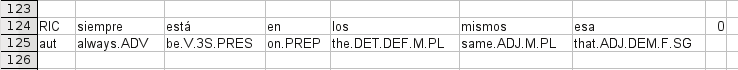
\includegraphics[scale=0.6]{cells.png}
  \end{figure}
\end{frame}

\begin{frame}
\frametitle{\begin{small}\insertframenumber/\inserttotalframenumber\end{small} Accessibility}
\begin{itemize}
\item Interactive webpages (\textit{siarad.org.uk})
% easier mining of the data, no need to install CLAN
  \begin{figure}[h]
  \centering
  %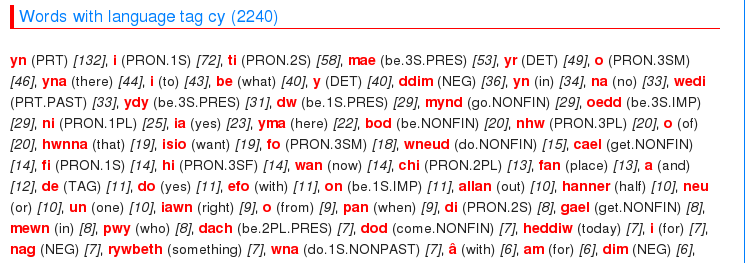
\includegraphics[scale=0.5]{frequency.png}
  \end{figure}
% click on gael, and you get ...
\end{itemize}
\end{frame}

\begin{frame}
\frametitle{\begin{small}\insertframenumber/\inserttotalframenumber\end{small} Accessibility}
  \begin{figure}[h]
  \centering
  %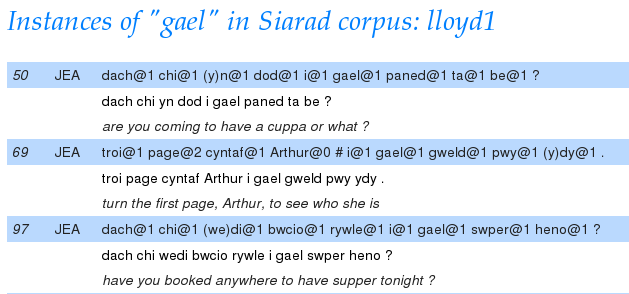
\includegraphics[scale=0.5]{context.png}
  \end{figure}
\begin{itemize}
\item Interface to CLAN queries
% already a very good web interface, but you could aim this more at beginners, with potted queries
\end{itemize}
\end{frame}

\subsection{Data-mining}

\begin{frame}
\frametitle{\begin{small}\insertframenumber/\inserttotalframenumber\end{small} Data-mining}
\begin{itemize}
\item Utterance profiling
  \begin{columns}
  \begin{column}{0.7\textwidth}
    \begin{figure}[h]
    \centering
    %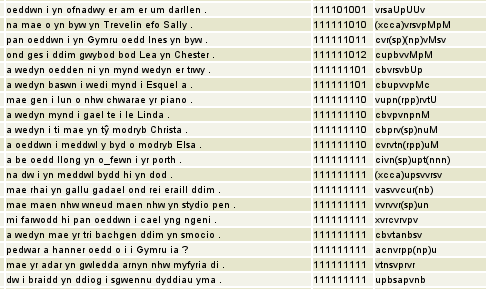
\includegraphics[scale=0.5]{fingerprint.png}
    \end{figure}
  \end{column}
  \begin{column}{0.3\textwidth}
    \begin{figure}[h]
    \centering
    %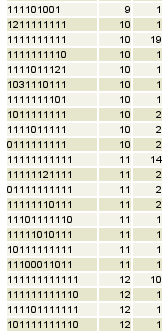
\includegraphics[scale=0.5]{profile.png}
    \end{figure}
  \end{column}
  \end{columns}
\end{itemize}
\end{frame}

\begin{frame}
\frametitle{\begin{small}\insertframenumber/\inserttotalframenumber\end{small} Data-mining}
\begin{itemize}
\item Easier or more detailed statistical analysis
\item N-gram generation (2- or 3-word collocations)
\item Input to statistical machine translation
\end{itemize}
\end{frame}




\end{document}